\chapter{探测器蒙特卡洛模拟}
\label{chapter:background}

为了寻找NLDBD这个极其稀有的事件,一个极低本底的探测环境是PandaXIII实验需要着重解决的问题。所以为了能够在探测器实际建造之前细致的研究探测器结构和材料对本底水平的研究,我们使用Geant4\supercite{Agostinelli:2002hh}作为主要的蒙特卡洛模拟框架,构建了模拟器的模型。通过这个模型我们可以细致的研究探测器各个组件以及环境对实验本底的贡献,并根据这些数据来调节探测器的各种各样参数以达成实验的设计目标。具体的模拟细节如下列小节所述。

\section{目标元素及模拟工具}

因为探测器的铜壁相对较厚,而且铜壁的材料可以制作的较为纯净,在考虑到铜壁的屏蔽效应后,来自铜壁外的$\alpha$射线和$\beta$射线基本不可能到达探测器内部的灵敏区域,所以需要主要考虑到的本底辐射为探测器铜壁内部原件的各种辐射以及环境和材料中的$\gamma$射线。因为$^{136}$Xe的NLDBD事件释放出来的总能量$Q_{\beta\beta}=2458$keV,探测器设计的相对能量分辨率是3\%FWHW(半高全宽),因而我们定义能量窗口($Q_{\beta\beta}-2\sigma$, $Q_{\beta\beta}+2\sigma$)为能量敏感区域(Region Of Interest, ROI),其中$\sigma$为探测器在$Q_{\beta\beta}$处的绝对能量分辨率。计算可得ROI范围为2395keV到2520keV,所以衰变能量落在这个能量范围附近的元素便是我们感兴趣的元素。

根据各种放射性元素的衰变能量和在自然界中的丰度,再结合既往有关$^{136}$Xe的
NLDBD实验研究结果可以得到,我们关心的主要本底来自于$^{214}$Bi的gamma衰变,其能量为2447.8keV,以及来自于$^{208}$Tl的gamma衰变,其能量为2615.keV。这两种元素分别属于$^{238}$U和$^{232}Th$的衰变链中,而这两种放射性元素在自然界中大量的存在,绝大多数的材料都或多或少的含有它们。除了这两种元素,$^{60}$Co可能会释放出1.33MeV和
1.17MeV的$\gamma$射线,虽然两者和能量约为2.5MeV,但是这两个射线相对独立,同时落在探测器敏感区域内的概率不大,在加上读出窗口的限制$^{60}$Co对实验的影响会变得更小,因而在后续的模拟中它并没有被着重研究。表\ref{tab:activities}给出了构建探测器的原料中Th,U的放射性活度。
\renewcommand\arraystretch{1.4}
\begin{table*}[tbh]
    \centering
    \begin{tabular*}{0.75\textwidth}{@{\extracolsep{\fill}}cccc}
        \hline
        \hline
        \multirow{2}{*}{\textbf{材料}} & \multicolumn{3}{c}{\textbf{放射性活度 ($\mu$Bq/kg)}}
      \\
                                   & $^{232}$Th & $^{238}$U  & $^{60}$Co \\ \hline
      铜                       & 0.2        &   0.75     &     100     \\
      PTFE                         & 0.1        &   4.94      &    -      \\
      不锈钢              & 0.32$\times$10$^3$          &    0.5$\times$10$^3$      &     2.6$\times$10$^3$     \\
      超纯水                          & 0.04          &     0.12      &     -     \\
      混泥土                     & 9.9$\times$10$^6$          &    4.4$\times$10$^6$   &    -    \\
        \hline
        \hline
    \end{tabular*}
    \caption{不同材料的放射性活度表。铜和PTFE的活动数据来自于文献\cite{Abgrall:2016cct},不锈钢的数据来自于文献\cite{LZ_CDR},超纯水的数据来自于PandaXIII的中期报告\cite{cdr},混泥土的数据来自于文献\cite{Zeng2014}。}
    \label{tab:activities}
  \end{table*}
  

PandaXIII模拟工作中我们使用了Geant4软件作为蒙特卡洛模拟框架。Geant4是由
CERN开发的基于C++的蒙特卡罗应用包,它主要用于模拟粒子在物质中发生的各种物理过程。它内置了做粒子追踪所需要的完整方法包括径迹追踪,探测器几何构建,物理模型和数据等等,其中物理过程中包含了极大能量尺度下各种粒子之间的相互作用,材料和元素的数据。该软件被广泛的应用在了核物理,高能物理,医学研究等等领域。

PandaXIII实验在Geant4软件框架的基础上二次开发了两个模拟框架以满足复杂的模拟需求,分别被称作BambooMC和RestG4。BambooMC是由上海交通大学基于
PandaXII暗物质实验的模拟需求开发改进而成,后者是REST软件\supercite{tomas2013development}的一个模块。我们使用这两种框架独立进行了背景模拟工作,并对两者的结果做了交叉检查以确保结果的正确性。本文中的模拟工作都是由BambooMC模拟框架完成的。

\section{探测器结构及本底来源}
\begin{figure}[tbh]
    \centering
    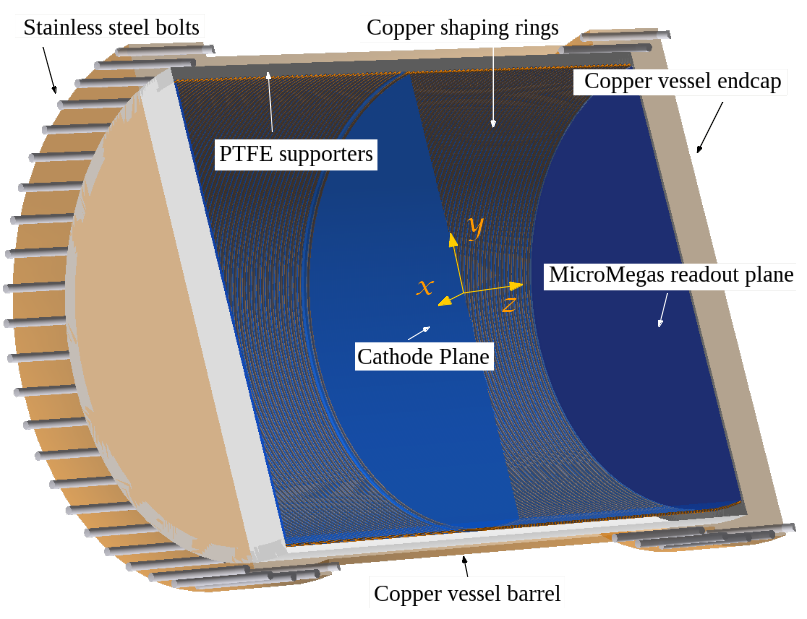
\includegraphics[width=0.4\columnwidth]{pic/fig3.png}
    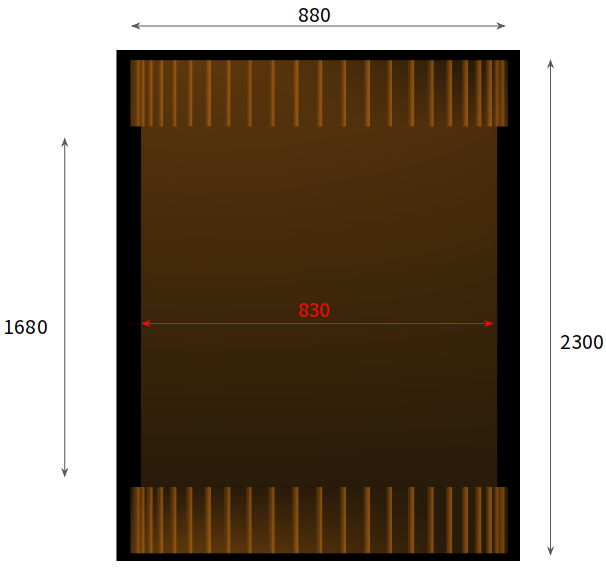
\includegraphics[width=0.4\columnwidth]{pic/fig5.png}
    \caption{左图:Geant4中PandaXIII背景模拟时间漂移室示意图\supercite{cnn},探测器被演奏平面切开。右图:铜罐结构的正视图以及外围尺寸。}
    \label{fig:detector_bamboomc}
\end{figure}

使用BambooMC构建出来的探测器结构如图\ref{fig:detector_bamboomc}所示。铜罐是由一个有法兰的圆柱体和两端的铜盖组成,每侧的铜盖和铜罐之间使用48个不锈钢螺钉铆和,铜罐壁厚度为3厘米,两端铜盖厚度为15厘米。在铜罐内部就是时间漂移室的主体结构,是由5cm厚度PTFE材料的作为支撑,延Z方向镶嵌99个管状圆形铜环组成的场笼,用于形成均匀的延Z方向的漂移电场。两个Micromegas读出平面放置在探测器的两端,同时中心的圆形铜极板将探测器分为上下两个漂移室。探测器主要原件的尺寸可以参照表\ref{tab:parameters_geometry}。
\begin{table*}[thb]
    \begin{center}
        \begin{tabular*}{0.75\textwidth}{@{\extracolsep{\fill}}ccccc}
        \hline
        \hline
        \textbf{组件} & \textbf{参数} & \textbf{值} & \textbf{材料} & \textbf{质量} \\ \hline
        \multirow{3}{*}{铜罐} & 内径 & 80\,cm & \multirow{3}{*}{铜} & \multirow{3}{*}{3438 kg} \\
                    & 高度 & 200\,cm &  &    \\   
                    & 壁厚 & 3\,cm &  &    \\\hline
        \multirow{2}{*}{铜盖} & 直径 & 88\,cm & \multirow{2}{*}{铜} & \multirow{2}{*}{3320 kg} \\
                    & 厚度 & 15\,cm &  &    \\\hline
        \multirow{2}{*}{螺钉} & 直径 & 1.4\,cm & \multirow{2}{*}{不锈钢} & \multirow{2}{*}{230.1 kg} \\
                    & 高度 & 40\,cm &  &    \\\hline
        \multirow{4}{*}{场笼} & 内径 & 75\,cm & \multirow{3}{*}{PTFE} & \multirow{3}{*}{1042 kg} \\
                    & 高度 & 200\,cm &  & \\ 
                    & 厚度 & 5\,cm &  & \\ 
                    & 铜环个数 & 99 &    \multirow{1}{*}{铜}  & 118.2 kg \\\hline
        中心极板 & 厚度   &   50\,$\mu$m     &   \multirow{1}{*}{铜}  &    0.79 kg   \\   
        \hline
        \hline
        \end{tabular*}
        \caption{探测器组成部件的几何参数,材料以及质量表。\supercite{cdr}}
        \label{tab:parameters_geometry}
    \end{center}
\end{table*}
  
探测器铜罐内填充了200kg的氙气与TMA混合气体,总体气压为10bar,被放置在中国锦屏地下实验室中的水池中。下列详细描述了探测器各个部分对本地的贡献:


\begin{description}
    \item[铜罐] 测试
    \item[电子学] 测试
\end{description}


\section{探测器响应及读出触发}

% vim:ts=4:sw=4
